%&pdflatex
\documentclass{standalone}
\usepackage{tikz}
\usetikzlibrary{arrows}
\usetikzlibrary{shapes}

\begin{document}

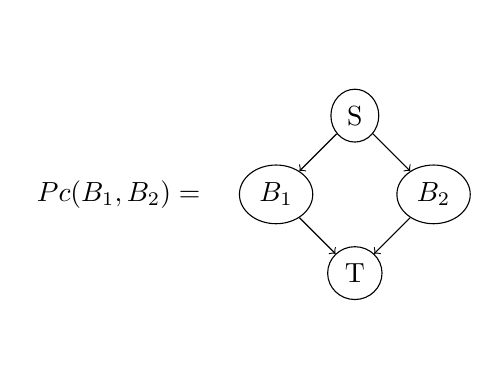
\begin{tikzpicture}
    \node (dummy) at (2,4) {};
    \node (dummy2) at (2, 0) {};
    \node (Pc) at (0,2) { \(Pc(B_1,B_2)=\)};
    \node[draw, ellipse] (S) at (3,3) {S};
    \node[draw, ellipse] (B1) at (2, 2) {\( B_1 \)};
    \node[draw, ellipse] (B2) at (4, 2) {\( B_2 \)};
    \node[draw, ellipse] (T) at (3, 1) {T};

    \draw[->] (S) to (B1);
    \draw[->] (S) to (B2);
    \draw[->] (B1) to (T);
    \draw[->] (B2) to (T);
\end{tikzpicture}

\end{document}



